\chapter[Cost of Capital: Risk-Free Rate, Risk Premia, Beta, Cost of Debt]{Cost of Capital:\\Risk-Free Rate, Risk Premia,\\Beta and Cost of Debt}\label{ch:coc}

\emph{Based on Lecture L07 (53 slides), in two parts: ``Cost of Capital -- Part 1: Risk-Free Rate and Risk Premia'' and ``Part 2: Risk Parameters and Cost of Financing''. Part Two of the course (workflow step: discount rate).}

% =====================================================================
\section*{PART 1 -- RISK-FREE RATE AND RISK PREMIA}
\addcontentsline{toc}{section}{Part 1 -- Risk-Free Rate and Risk Premia}

\section{Business Valuation Methods: DCF Models}

DCF models are based on the \textbf{present value approach}: the value of any asset is the present value of the expected future cash flows on it.
\begin{keybox}[DCF value]
\[
V_t=\sum_{s=t+1}^{n}\frac{\mathbb{E}_t[\text{FCF}_s]}{(1+r)^{s-t}}
\]
$n$: expected life of the assets (usually $n=\infty$ for a business); FCF$_s$: expected free cash flow in period $s$; $r$: discount rate reflecting the riskiness of the FCFs, aka the \textbf{cost of capital}.
\end{keybox}

\section{Cost of Capital}

\subsection{General Setup for Valuation}
\begin{itemize}
  \item We need to know which \textbf{discount rate} to use to compute the PV of the expected cash flows generated by the assets (or by a firm's equity).
  \item That discount rate is the \textbf{opportunity cost of capital}: the rate an investor requires to ``hold'' the expected cash flows generated by the assets.
  \item The required return for holding all the future cash flows of a firm is its \textbf{Weighted Average Cost of Capital (WACC)}.
  \item Why? \textbf{Modigliani--Miller}: if you buy all the securities issued by a firm (debt, equity, any other), you own 100\% of the firm's assets and thus of the total (free) cash flows. You also own a portfolio whose expected return is the weighted average of the expected returns on those securities, weighted by their proportion in the capital structure.
\end{itemize}

\subsection{WACC}
\begin{keybox}[WACC with three classes of securities]
\[
\text{WACC}=r_d(1-\tau_C)\frac{D}{D+E+S}+r_e\frac{E}{D+E+S}+r_s\frac{S}{D+E+S}
\]
$r_d$, $r_e$, $r_s$: expected returns on debt, equity and security $S$ (if any, e.g., preferred stock, hybrids); $\tau_C$: corporate tax rate; $D$, $E$, $S$: \textbf{market values}.
\end{keybox}
\slidefig{Warning: using the WACC implies making specific assumptions, which are not always warranted. In such cases you cannot use the WACC (see Chapters~\ref{ch:wacc}--\ref{ch:capstr}: WACC assumes a constant leverage ratio).}

\subsection{Risk and Return Models}
Leading models of risk and return derive a security's expected return as the sum of the \textbf{risk-free rate} (the rate investors can earn on riskless investments) and the \textbf{risk premium(s)} they require for holding risky assets.
\begin{keybox}[CAPM and multifactor models]
\textbf{CAPM}: \quad $\mathbb{E}[r_e]=r_f+\beta\cdot\mathbb{E}[r_m-r_f]$ \quad -- only one source of risk, the market portfolio (expected return $\mathbb{E}[r_m]$); $\beta$ is the exposure to it.\\[4pt]
\textbf{Multifactor}: \quad $\mathbb{E}[r_e]=r_f+\sum_{i=1}^{n}\beta_i\cdot\mathbb{E}[r_i-r_f]$ \quad -- multiple sources of risk $i$; $\beta_i$ are the exposures.
\end{keybox}

% =====================================================================
\section{Estimating the Risk-Free Rate}

\subsection{Principles}
On a risk-free asset, \textbf{expected return $=$ actual return}. A risk-free investment has \textbf{no default risk} and \textbf{no reinvestment (rollover) risk}.
\begin{enumerate}
  \item \textbf{Time horizon.} At any point in time, borrowers face different rates for cash flows of different maturities (\emph{term structure}). Match the \textbf{maturity} of the asset being valued with the maturity of the risk-free government bond rate.
  \item \textbf{Not all government securities are risk-free.} Some governments face default risk, so their bond rates are not risk-free; this is also true if they borrow in a currency other than their own.
  \item \textbf{Consistency principle.} Nominal cash flows require nominal risk-free rates; the \textbf{currency} of the cash flows must be the currency of the risk-free rate.
\end{enumerate}

\subsection{Real vs Nominal Rates}
Under high and unstable inflation, valuation is often done in \textbf{real} terms $\Rightarrow$ make sure the cash flows reflect real growth, not growth from price inflation. How to estimate the real expected return:
\begin{enumerate}
  \item \textbf{``Subtracting'' inflation} (standard approach):
  \[
  r_{f,\text{real}}\approx r_{f,\text{nominal}}-i\quad(\text{only for low } i)\qquad\qquad r_{f,\text{real}}=\frac{1+r_{f,\text{nominal}}}{1+i}-1
  \]
  \item \textbf{Inflation-indexed Treasuries (TIPS)}: they offer a guaranteed real return (only for the US: low and stable $i$).
  \item \textbf{No financial-market frictions} (capital flows freely): no differences in real $r_f$ across countries $\Rightarrow$ use TIPS for all countries.
  \item \textbf{Financial-market frictions}: the expected long-term real $r_f$ should equal the expected long-term growth ($g$).
\end{enumerate}
\begin{exbox}[Illustration (not on slides)]
Nominal $r_f=10\%$, expected inflation $i=6\%$: approximation $10\%-6\%=4\%$; exact $\frac{1.10}{1.06}-1=3.77\%$. The gap grows with inflation, which is why the approximation holds only for low $i$.
\end{exbox}

\subsection{Sovereign Default Spreads: Risk-Free Rate in a Local Currency}
\begin{enumerate}
  \item \textbf{Local-currency government bond}:
  \begin{enumerate}[label=(\alph*)]
    \item \textbf{Default spread approach}: \quad $r_f\ \text{in LC}=\text{Govt bond rate (LC)}-\text{Default spread}$.\\ The default spread comes from the USD credit spread (USD bonds of that government); for countries without USD bonds, use the average spread of countries in the same rating class.
    \item \textbf{Insurance (CDS) approach}: \quad $r_f\ \text{in LC}=\text{Govt bond rate (LC)}-\text{CDS spread}$.
  \end{enumerate}
  \item \textbf{Build-up approach}: if there is no traded government bond in local currency,\\ \quad Build-up $r_f=$ expected inflation $+$ expected long-term real growth rate.
  \item \textbf{Derivatives markets} (no frictions): use \textbf{covered interest parity} to back out $r_f$ in LC:
  \[
  \text{Forward rate}_{LC,USD}=\text{Spot rate}_{LC,USD}\times\frac{1+r_{f,LC}}{1+r_{f,USD}}
  \]
  \item \textbf{Risk-free rate conversion} (frictions): use \textbf{uncovered interest parity} (relative inflation):
  \[
  (1+r_{f,USD})=(1+r_{f,LC})\,\frac{1+\text{Expected inflation}_{USD}}{1+\text{Expected inflation}_{LC}}
  \]
\end{enumerate}

\subsection{Data (January 2022)}

\begin{center}
\scriptsize
\begin{tabular}{@{}lr@{\hspace{6pt}}lr@{\hspace{6pt}}lr@{}}
\toprule
\textbf{Currency} & \textbf{Govt bond} & \textbf{Currency} & \textbf{Govt bond} & \textbf{Currency} & \textbf{Govt bond}\\
\midrule
Australian \$ & 1.67\% & Indian Rupee & 6.45\% & Qatari Dinar & 2.11\%\\
\textcolor{keyred}{Brazilian Reai} & \textcolor{keyred}{10.31\%} & Indonesian Rupiah & 1.02\% & Romanian Lev & 5.21\%\\
British Pound & 0.97\% & Israeli Shekel & 1.02\% & Russian Ruble & 8.42\%\\
Bulgarian Lev & 0.70\% & Japanese Yen & 0.07\% & Singapore \$ & 1.67\%\\
Canadian \$ & 1.43\% & Kenyan Shilling & 12.55\% & South African Rand & 9.35\%\\
Chilean Peso & 5.72\% & Korean Won & 2.26\% & Swedish Krona & 0.21\%\\
Chinese Yuan & 2.85\% & Malaysian Ringgit & 3.59\% & Swiss Franc & $-0.14\%$\\
Colombian Peso & 8.14\% & Mexican Peso & 7.56\% & Taiwanese \$ & 0.69\%\\
Croatian Kuna & 0.63\% & Nigerian Naira & 12.61\% & Thai Baht & 1.95\%\\
Czech Koruna & 2.98\% & Norwegian Krone & 1.72\% & Turkish Lira & 23.33\%\\
Danish Krone & 0.10\% & NZ \$ & 2.33\% & US \$ & 1.51\%\\
Euro & $-0.18\%$ & Pakistani Rupee & 11.54\% & Vietnamese Dong & 2.12\%\\
HK \$ & 1.45\% & Peruvian Sol & 5.87\% & Zambian kwacha & 31.50\%\\
Hungarian Forint & 4.58\% & Philippine Peso & 4.90\% & & \\
Iceland Krona & 4.15\% & Polish Zloty & 3.66\% & & \\
\bottomrule
\end{tabular}
\end{center}

\begin{center}
\small
\begin{minipage}[t]{0.47\textwidth}
\centering
\textbf{Sovereign default spreads from \$ (or \euro) bonds}\\[3pt]
\begin{tabular}{@{}lrrr@{}}
\toprule
Country & \$ bond & $r_f$ & Spread\\
\midrule
Peru & 3.66\% & 1.51\% & 2.15\%\\
\textcolor{keyred}{Brazil} & \textcolor{keyred}{3.70\%} & \textcolor{keyred}{1.51\%} & \textcolor{keyred}{2.19\%}\\
Colombia & 2.33\% & 1.51\% & 0.82\%\\
Poland & 1.80\% & 1.51\% & 0.29\%\\
Turkey & 5.43\% & 1.51\% & 3.92\%\\
Mexico & 2.01\% & 1.51\% & 0.50\%\\
Russia & 2.48\% & 1.51\% & 0.97\%\\
\multicolumn{4}{@{}c}{\emph{Euro bonds}}\\
Bulgaria & 1.00\% & $-0.18\%$ & 1.18\%\\
\bottomrule
\end{tabular}
\end{minipage}\hfill
\begin{minipage}[t]{0.5\textwidth}
\centering
\textbf{Rating-based default spreads}\\[3pt]
\scriptsize
\begin{tabular}{@{}llr@{\hspace{8pt}}llr@{}}
\toprule
S\&P & Moody's & Spread & S\&P & Moody's & Spread\\
\midrule
AAA & Aaa & 0.00\% & B+ & B1 & 3.83\%\\
AA+ & Aa1 & 0.34\% & B & B2 & 4.68\%\\
AA & Aa2 & 0.42\% & B$-$ & B3 & 5.53\%\\
AA$-$ & Aa3 & 0.51\% & CCC+ & Caa1 & 6.38\%\\
A+ & A1 & 0.60\% & CCC & Caa2 & 7.66\%\\
A & A2 & 0.72\% & CCC$-$ & Caa3 & 8.51\%\\
A$-$ & A3 & 1.02\% & CC+ & Ca1 & 10.21\%\\
BBB+ & Baa1 & 1.36\% & CC & Ca2 & 12.88\%\\
BBB & Baa2 & 1.62\% & CC$-$ & Ca3 & 14.50\%\\
BBB$-$ & Baa3 & 1.87\% & C+ & C1 & 15.50\%\\
BB+ & Ba1 & 2.13\% & C & C2 & 17.00\%\\
\textcolor{keyred}{BB} & \textcolor{keyred}{Ba2} & \textcolor{keyred}{2.56\%} & C$-$ & C3 & 19.00\%\\
BB & Ba3 & 3.06\% & & & \\
\bottomrule
\end{tabular}
\end{minipage}
\end{center}

\begin{figure}[H]
\centering
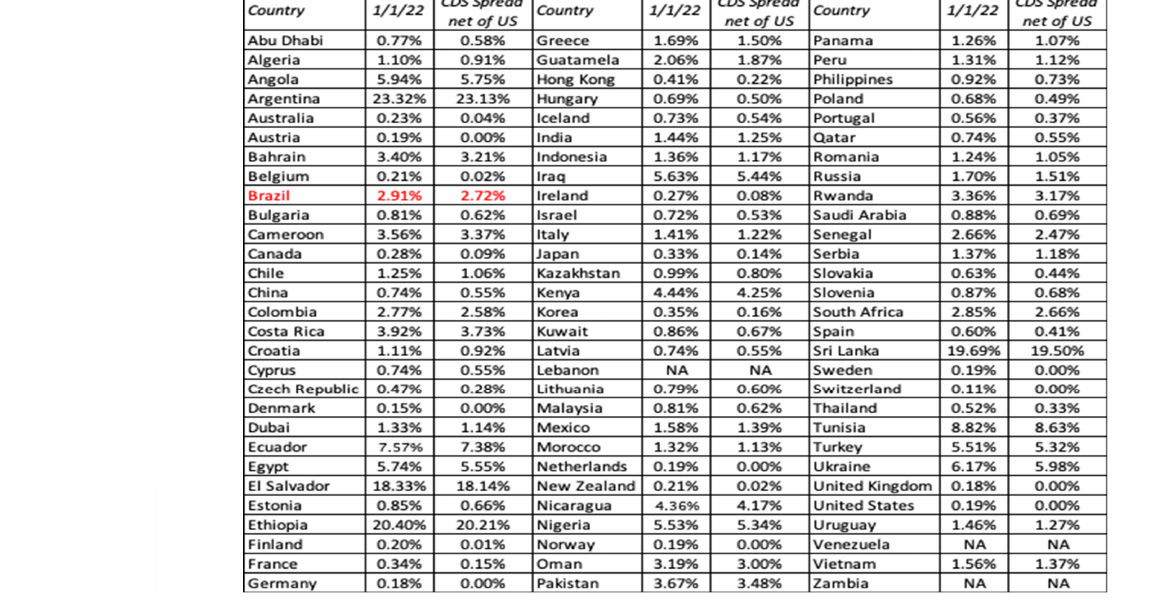
\includegraphics[width=0.85\textwidth]{L07_slide14.png}
\caption{CDS spreads by country, January 2022 (slide screenshot). Brazil: CDS 2.91\%, net of the US CDS 2.72\%.}
\end{figure}

\begin{exbox}[Test 3 (slide): risk-free rate in a currency -- Brazil]
The Brazilian government bond rate in nominal Reais on 1 January 2022 was 10.31\%. Three approaches to a nominal-Real $r_f$:
\begin{enumerate}
  \item \textbf{Government bond spread}: the 2032 USD-denominated Brazilian bond has a spread of 2.19\% over the US T-bond (3.70\% $-$ 1.51\%):\quad $r_f=10.31\%-2.19\%=\mathbf{8.12\%}$.
  \item \textbf{CDS spread}: Brazil's CDS spread net of the USD CDS spread was 2.72\%:\quad $r_f=10.31\%-2.72\%=\mathbf{7.59\%}$.
  \item \textbf{Rating-based spread}: Brazil had a Ba2 Moody's rating in LC; the spread for that class is 2.56\%:\quad $r_f=10.31\%-2.56\%=\mathbf{7.75\%}$.
\end{enumerate}
\end{exbox}

% =====================================================================
\section{Estimating the Equity Risk Premium (ERP)}

\subsection{Definitions}
\begin{itemize}
  \item \textbf{ERP}: the premium a \textbf{well-diversified marginal investor} requires to hold the market portfolio rather than a risk-free asset.
  \item \textbf{Historical ERP}: the premium stocks have \textbf{historically} earned over riskless securities over long periods. Implicit assumption: history can forecast the future.
  \item \textbf{Implied ERP}: the \textbf{forward-looking} premium implicitly priced in the \textbf{current} stock-market level, given expected aggregate cash flows and risk-free rates (see Martin, 2017, QJE). Implicit assumption: the market, overall and on average, is correctly priced.
\end{itemize}

\subsection{Peso Problems}
\begin{itemize}
  \item What about rare shocks? Also called \textbf{peso problems} or dark swans; very important for academics and practitioners.
  \item Answer: they account for \textbf{at most 1--2\%} of the historical equity premium. Not unimportant, and \textbf{insurable with index options}. Other long-run decline problems are harder to insure.
\end{itemize}

\subsection{Historical Risk Premium (HRP) Approach -- US}
Estimates are sensitive to:
\begin{enumerate}
  \item \textbf{Time period}: the ERP is time-varying; different periods give different measures; shorter periods have higher standard errors.
  \item \textbf{Choice of risk-free security}: T-bills (short term) vs T-bonds (long term). With an \textbf{upward-sloping} term structure, the ERP is \textbf{larger} when measured over short-term risk-free assets. Must be consistent with the $r_f$ used in the cost of capital.
  \item \textbf{Arithmetic vs geometric average}: \textbf{arithmetic} when returns are serially uncorrelated and the ERP estimate is for next year; \textbf{geometric} when returns are serially correlated (Fama--French 1988), adjusting for the long-term view (although we use 1-period models for the cost of capital).
\end{enumerate}
Even after the least-biased choices there are caveats:
\begin{enumerate}
  \item \textbf{Noisy estimates}: over 1928--2019 (about 90 years), with a 20\% annual standard deviation of returns, the standard error is $\geq2\%$:
  \[
  \text{Standard error in premium}\approx\frac{20\%}{\sqrt{90}}=2.1\%
  \]
  The implied standard deviation of equities rose to almost 50\% in the last quarter of 2008: think of the consequences for HRP if this volatility persisted.
  \item \textbf{Survivorship bias}: using 20th-century US data samples only the market that ``survived'' and was among the most successful.
\end{enumerate}
\begin{keybox}
There is a \textbf{trade-off between standard errors and survivorship bias}.
\end{keybox}
\begin{addbox}
Arithmetic $\geq$ geometric average always (e.g., returns $+50\%$, $-50\%$: arithmetic $0\%$, geometric $\sqrt{1.5\times0.5}-1=-13.4\%$). With 20 years instead of 90, the standard error would be $20\%/\sqrt{20}=4.5\%$, larger than the premium itself.
\end{addbox}

\subsection{HRP Approach -- Other Markets: Modified Historical Risk Premium}
\begin{keybox}[Modified historical risk premium]
\[
\text{ERP}=\text{Base premium for mature equity markets}+\text{Country premium}
\]
\end{keybox}
\begin{enumerate}
  \item \textbf{Base ERP} for a mature market: the US is the best available reference (4.72\% at end-2021).
  \item \textbf{Should there be a country premium?} Some argue country risk is fully diversifiable (open markets); Stulz (1999) argues it is not always diversifiable (segmented markets and/or cross-country correlation); Damodaran: add a \textbf{country risk premium (CRP)} when estimating the cost of capital for non-US markets.
  \item \textbf{How to estimate it?} Measure the \textbf{absolute country risk} and the firm's \textbf{exposure} to it.
\end{enumerate}

\subsection{CRP Approach 1: Default Risk Spreads}
CRP $=$ default spread of the bond issued by the country, but only if it is denominated in a currency for which a default-free entity exists. Two ways:
\begin{align*}
\text{(1)}\quad r_{e,USD}&=r_f+\beta\cdot\text{ERP}_{US}+\text{Default spread}\\
\text{(2)}\quad r_{e,USD}&=r_f+\beta\cdot(\text{ERP}_{US}+\text{Default spread})
\end{align*}
Shortcomings: (a) rating agencies lag markets in responding to changes in CRP; (b) a focus on default risk may obscure other risks for equity markets. Solutions: (a) use CDS spreads over a long period (e.g., 10 years); (b) use other risk measures: insurance prices, country scores (The Economist), or a CRP built up from fundamentals; (c) correct the default spread by the relative standard deviation.

\subsection{CRP Approach 2: Relative Standard Deviation}
The CRP is based on the volatility of market $X$ relative to the US market:
\[
\text{Relative SD}_X=\frac{\sigma_X}{\sigma_{US}}\qquad \text{ERP}_X=\text{ERP}_{US}\times\text{Relative SD}_X\qquad \text{CRP}_X=\text{ERP}_X-\text{ERP}_{US}
\]
Then use ERP$_X$ to estimate $r_e$. Shortcomings: (a) markets differ in structure and liquidity, which affects volatility; (b) some risky emerging markets have low volatility because of illiquidity; (c) currency differences (USD vs LC). Solutions: (a--b) examine the market structure and liquidity carefully; (c) compute USD-denominated returns to estimate the volatility of market $X$.

\subsection{CRP Approach 3: Default Spreads and Relative Standard Deviation}
\begin{keybox}
\[
\text{CRP}_X=\text{Country default spread}\times\frac{\sigma_{\text{Equity},X}}{\sigma_{\text{Bonds},X}}
\]
then (a) $r_{e,USD}=r_f+\beta\cdot\text{ERP}_{US}+\text{CRP}_X$ or (b) $r_{e,USD}=r_f+\beta\cdot(\text{ERP}_{US}+\text{CRP}_X)$.
\end{keybox}
Shortcomings and solutions are similar to the two previous approaches.
\begin{exbox}[Illustration (not on slides)]
Brazil: default spread 2.56\%, $\sigma_{\text{equity}}=30\%$, $\sigma_{\text{bonds}}=20\%$ $\Rightarrow$ CRP $=2.56\%\times1.5=3.84\%$. With $r_f=1.51\%$, ERP$_{US}=4.24\%$, $\beta=1.2$:\\
(a) $r_e=1.51\%+1.2\times4.24\%+3.84\%=10.44\%$; \quad (b) $r_e=1.51\%+1.2\times(4.24\%+3.84\%)=11.21\%$.\\
Relative-SD approach with $\sigma_{BR}/\sigma_{US}=1.6$: ERP$_{BR}=4.24\%\times1.6=6.78\%$, CRP $=2.54\%$.
\end{exbox}

\subsection{CRP: Exposure}
Three ways to bring the CRP into $r_e$, given the link between returns in LC and USD:
\[
r_{e,LC}=\left[(1+r_{e,USD})\cdot\frac{1+i_{LC}}{1+i_{USD}}\right]-1
\]
\begin{enumerate}
  \item \textbf{Every company in the country is equally exposed}: $r_{e,USD}=r_f+\beta\cdot\text{ERP}_{US}+\text{CRP}_{X}$ (implicit when using the local government's dollar borrowing rate as $r_f$).
  \item \textbf{Exposure to country risk $=$ exposure to market risk}: $r_{e,USD}=r_f+\beta\cdot(\text{ERP}_{US}+\text{CRP}_{X})$ (country risk is a portion of market risk).
  \item \textbf{Country risk as a separate factor}, firm-specific exposure $\lambda$: $r_{e,USD}=r_f+\beta\cdot\text{ERP}_{US}+\lambda\cdot\text{CRP}_{X}$ (multifactor model).
\end{enumerate}

\subsection{ERP Estimation Procedure and Implied ERP (January 2022)}

\begin{figure}[H]
\centering
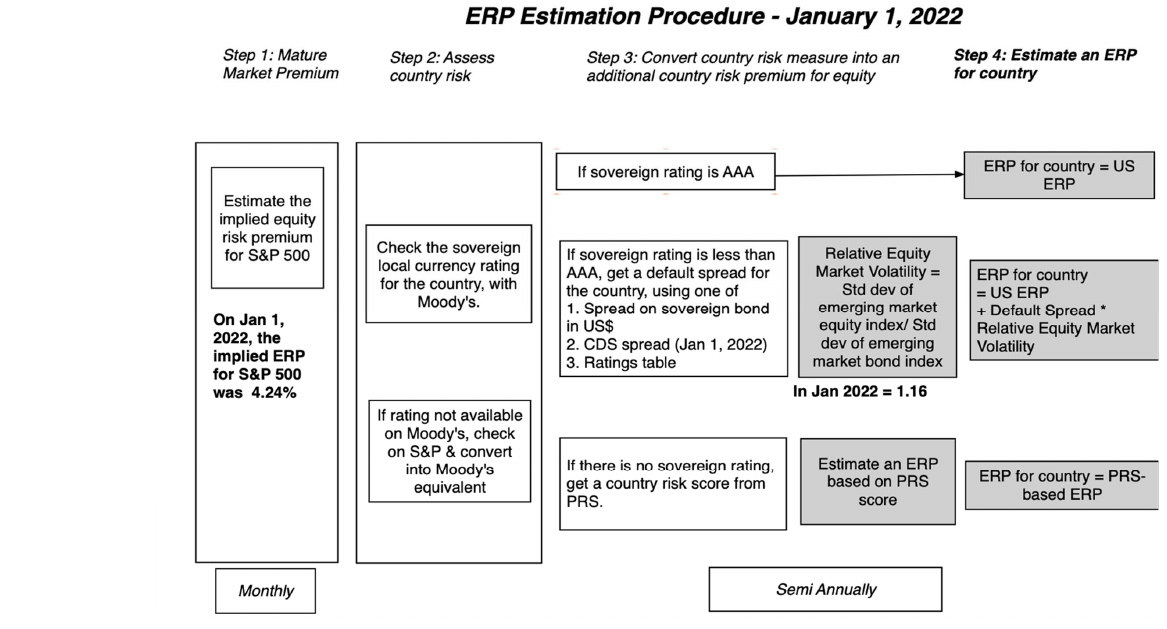
\includegraphics[width=0.9\textwidth]{L07_slide27.png}
\caption{ERP estimation procedure, 1 January 2022 (slide screenshot). Step 1: implied ERP for the S\&P 500 (4.24\%). Step 2: sovereign local-currency rating (Moody's; else S\&P or PRS score). Step 3: if the rating is below AAA, a default spread (sovereign \$ bond, CDS or ratings table) times the relative equity-market volatility (std dev of emerging-market equity index / std dev of emerging-market bond index $=1.16$ in January 2022). Step 4: ERP for the country $=$ US ERP $+$ default spread $\times$ relative equity-market volatility (or the PRS-based ERP).}
\end{figure}

\begin{figure}[H]
\centering
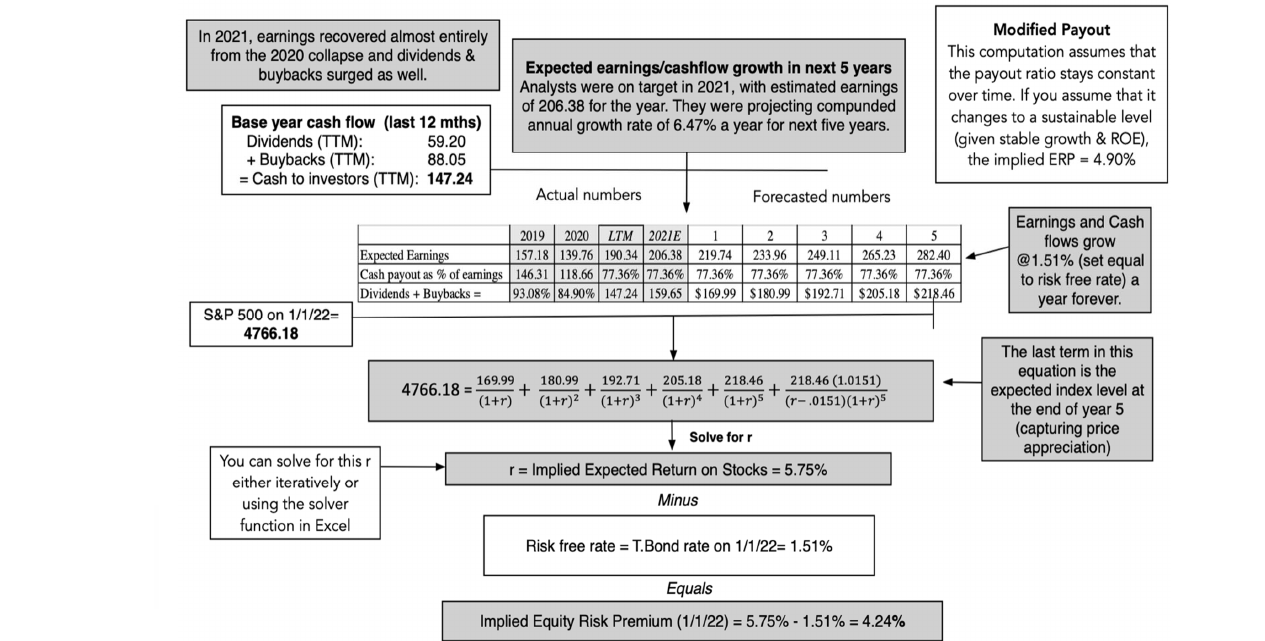
\includegraphics[width=0.9\textwidth]{L07_slide28.png}
\caption{Implied ERP, January 2022 (slide screenshot).}
\end{figure}

\begin{exbox}[Implied ERP: the computation step by step]
\begin{itemize}[leftmargin=*]
  \item Base-year cash to investors (last 12 months): dividends 59.20 + buybacks 88.05 $=$ \textbf{147.24}.
  \item Expected earnings grow at 6.47\% per year for 5 years (analysts); cash payout stays at 77.36\% of earnings $\Rightarrow$ cash flows: 169.99, 180.99, 192.71, 205.18, 218.46.
  \item After year 5, cash flows grow at 1.51\% ($=r_f$) forever.
  \item Solve for $r$ so that the index level equals the PV:
  \[
  4{,}766.18=\frac{169.99}{1+r}+\frac{180.99}{(1+r)^2}+\frac{192.71}{(1+r)^3}+\frac{205.18}{(1+r)^4}+\frac{218.46}{(1+r)^5}+\frac{218.46\times1.0151}{(r-0.0151)(1+r)^5}
  \]
  The last term is the expected index level at the end of year 5. Solution (iteratively or with Excel's solver): $r=\mathbf{5.75\%}$ (we verify: 5.753\%).
  \item Implied ERP $=5.75\%-1.51\%=\mathbf{4.24\%}$.
  \item \textbf{Modified payout}: if the payout moves to a sustainable level (given stable growth and ROE), the implied ERP $=4.90\%$.
\end{itemize}
\end{exbox}

\subsection{Part 1 Takeaways}
\begin{itemize}
  \item The CAPM is a model of how risk is priced in capital markets.
  \item In the CAPM, idiosyncratic risk can be diversified away $\Rightarrow$ \textbf{only systematic risk is priced}.
  \item The CAPM is empirically rejected, but it is still widely used to estimate the cost of equity. We need 3 parameters:
  \begin{itemize}
    \item \textbf{risk-free rate}, typically the yield of a long-term government bond;
    \item \textbf{beta}, from historical monthly, weekly or daily returns; estimates are noisy (use comparable companies to improve precision); measure it over a period in which leverage and operations are stable;
    \item \textbf{ERP}, the expected return on a broad-based index in excess of the risk-free rate.
  \end{itemize}
  \item The estimates of beta, ERP and risk-free rate are \textbf{logically linked together}.
\end{itemize}

% =====================================================================
\section*{PART 2 -- RISK PARAMETERS AND COST OF FINANCING}
\addcontentsline{toc}{section}{Part 2 -- Risk Parameters and Cost of Financing}

\section{Estimating Beta}

\subsection{Historical Market Betas}
Regress stock returns on market returns:
\begin{keybox}[Regression beta]
\[
r_{it}=\alpha+\beta\cdot r_{mt}+\varepsilon_{it},\qquad \beta=\frac{\text{Cov}(r_i,r_m)}{\text{Var}(r_m)}=\frac{\sigma_{im}}{\sigma_m^2}
\]
$\alpha$ = intercept; $\beta$ = slope: the riskiness of the stock relative to the market.
\end{keybox}
\textbf{Jensen's alpha.} To reconcile the CAPM with the regression:
\[
\mathbb{E}[r_i]=r_f+\beta\cdot\mathbb{E}[r_m-r_f]=r_f(1-\beta)+\beta\cdot\mathbb{E}[r_m]
\]
Compare the regression $\alpha$ (ex post) with $r_f(1-\beta)$ (ex ante):
\begin{center}
\begin{tabular}{@{}ll@{}}
\toprule
$\alpha>r_f(1-\beta)$ & the stock did \textbf{better} than expected over the period\\
$\alpha=r_f(1-\beta)$ & the stock did as expected\\
$\alpha<r_f(1-\beta)$ & the stock did \textbf{worse} than expected\\
\bottomrule
\end{tabular}
\end{center}
\begin{keybox}[Blume's adjustment (e.g., Bloomberg)]
\[
\beta_{\text{Adj}}=\beta_{\text{Raw}}\cdot\tfrac{2}{3}+1.00\cdot\tfrac{1}{3}
\]
(betas tend to revert towards 1 over time). Example: raw $\beta=1.6\Rightarrow\beta_{\text{Adj}}=1.067+0.333=1.40$.
\end{keybox}
Shortcomings: high standard errors; the regression reflects the firm's business mix and leverage \textbf{over the regression period}, not the current ones; not available for private firms and not reliable for illiquid markets.

\textbf{Summary of problems}
\begin{enumerate}
  \item \textbf{Historical returns}: a longer period gives more observations but may introduce biases from structural changes in the firm/industry risk profile $\Rightarrow$ use a shorter period, \textbf{between 2 and 5 years}.
  \item \textbf{Return type}: stock and market returns should include capital gains \textbf{and dividends}; some sources use price changes only.
  \item \textbf{Frequency}: daily returns give more observations but bias betas because of the illiquidity of some stocks.
  \item \textbf{Market index}: with internationally diversified investors, it is increasingly common to estimate $\beta$ against international indices (e.g., MSCI).
\end{enumerate}
\textbf{Solutions}
\begin{enumerate}
  \item Modify the regression beta: change the index, the frequency of returns, the length of the period; reduce the biases (Dimson 1979; Scholes and Williams 1977).
  \item \textbf{Accounting betas}: regress changes in the firm's earnings on changes in market earnings. Problems: (i) earnings smoothing, (ii) non-operating accounting policies, (iii) earnings frequency (at most quarterly).
  \item \textbf{Bottom-up beta (often preferable)}: requires understanding the type of business(es), the business mix and the financial leverage of the firm. The beta of a portfolio is the value-weighted average of the betas:
  \[
  \beta_P=\beta_a\omega_a+\beta_b\omega_b=\beta_a\frac{A}{A+B}+\beta_b\frac{B}{A+B}\iff \beta_P=\sum_{i=1}^{n}\beta_i\,\omega_i
  \]
\end{enumerate}

\subsection{Bottom-Up Betas: Determinants}
\begin{center}
\small
\begin{tabularx}{\textwidth}{@{}>{\raggedright\arraybackslash}p{3.6cm}>{\raggedright\arraybackslash}X>{\raggedright\arraybackslash}X@{}}
\toprule
\textbf{Determinant} & \textbf{Rule (other things equal)} & \textbf{Implications}\\
\midrule
\multicolumn{3}{@{}l}{\emph{Beta of the firm (unlevered $\beta$)}}\\
Nature of product/service & The more \textbf{discretionary} the product or service, the higher the $\beta$ & Cyclical $>$ non-cyclical; luxury $>$ basic goods; high-priced $>$ low-priced goods; growth firms have higher $\beta$\\
Operating leverage (fixed costs as \% of total costs) & The greater the proportion of \textbf{fixed costs}, the higher the $\beta$ & Rigid cost structures / high infrastructure needs $>$ flexible ones; small $>$ large firms; young $>$ mature firms\\
\midrule
\multicolumn{3}{@{}l}{\emph{Beta of equity (levered $\beta$)}}\\
Financial leverage & The greater the proportion of \textbf{debt}, the higher the equity $\beta$ & Highly levered firms have higher $\beta$; equity $\beta=$ unlevered $\beta\times$ (adjustment)\\
\bottomrule
\end{tabularx}
\end{center}

\subsection{Bottom-Up Betas: Ideal World and Real World}
\textbf{Ideal world}: start with the $\beta$ of the business the firm is in $\to$ adjust it for the operating leverage of the firm to obtain the unlevered $\beta$ $\to$ use the firm's financial leverage to obtain the levered (equity) $\beta$. Two alternatives (as in Chapter~\ref{ch:wacc}):
\begin{align*}
\text{Constant } D/(D+E):&\quad \beta_l=\beta_u\left[1+\frac{D}{E}\right]\\
\text{Fixed \$ debt (Hamada)}:&\quad \beta_l=\beta_u\left[1+(1-\tau_C)\frac{D}{E}\right]
\end{align*}

\textbf{Real world -- five steps}
\begin{enumerate}
  \item Find the business(es) your firm operates in.
  \item Find publicly traded firms in each business and obtain their regression $\beta$. \textbf{Unlever} each one with its own $D/E$: $\beta_u=\beta_{\text{regression}}/(1+D/E)$ [or Hamada if using APV]. Take the (simple or cap-weighted) average/median of these unlevered betas. Relever using your firm's $D/E$ (for pure players only). \emph{Refinement}: adjust for differences in operating leverage and product characteristics between your firm and the comparables.
  \item Estimate how much value your firm derives from each business. \emph{Refinement}: revenues or operating income are often used as weights, but it is better to estimate the \textbf{value} of each business.
  \item Compute the weighted average of the unlevered betas of the businesses (step 2) with the weights of step 3: \textbf{bottom-up unlevered $\beta$}. \emph{Refinement}: if the business mix changes over time, change the weights year by year.
  \item Compute the levered (equity) $\beta$ with the firm's \textbf{market} $D/E$: $\beta_l=\beta_u(1+D/E)$ [or Hamada if using APV] (if debt is riskless). \emph{Refinement}: if $D/E$ is expected to change, the levered $\beta$ changes over time.
\end{enumerate}

\begin{exbox}[Illustration (not on slides): bottom-up beta of a two-business firm]
Business A: comparables' average regression $\beta=1.20$, average $D/E=0.50$ $\Rightarrow\beta_u=1.20/1.5=0.80$. Business B: $\beta=0.90$, $D/E=0.20\Rightarrow\beta_u=0.75$.\\
Value weights: A 60\%, B 40\% $\Rightarrow\beta_u=0.6\times0.80+0.4\times0.75=0.78$.\\
Firm's market $D/E=0.40$: $\beta_l=0.78\times1.40=\mathbf{1.092}$ (textbook) or, with $\tau=25\%$, Hamada $0.78\times(1+0.75\times0.4)=\mathbf{1.014}$.
\end{exbox}

\subsection{Bottom-Up Betas: Adjusting Financial Leverage}
\begin{keybox}[Three approaches]
\textbf{1. Hamada} ($\beta_D=0$, $D$ fixed in \$): \quad $\beta_L=\beta_U\left[1+(1-\tau_C)\frac{D}{E}\right]$\\[4pt]
\textbf{2. Textbook WACC} ($D/E$ fixed, $\beta_D=0$): \quad $\beta_L=\beta_U\left[1+\frac{D}{E}\right]$\\[4pt]
\textbf{3. Debt-adjusted} (debt carries market risk, $\beta_D\neq0$):
\begin{align*}
\beta_L&=\beta_U\left[1+(1-\tau_C)\frac{D}{E}\right]-\beta_D(1-\tau_C)\frac{D}{E}\quad\text{(\$ debt fixed)}\\
\beta_L&=\beta_U\left[1+\frac{D}{E}\right]-\beta_D\frac{D}{E}\quad(D/E\text{ fixed})
\end{align*}
\end{keybox}
While the debt-adjusted approach is desirable, \textbf{estimating $\beta_D$ is often challenging}.

\subsection{Bottom-Up Betas: Reasons to Use Them}
\begin{itemize}
  \item \textbf{Lower noise}: the standard error of a bottom-up $\beta$ is much lower than that of a single regression $\beta$:
  \[
  \text{Std error of bottom-up }\beta\approx\frac{\text{Average std error across }\beta\text{s}}{\sqrt{\#\text{ of firms in sample}}}
  \]
  e.g., average error 0.25 with 25 comparables $\Rightarrow0.25/5=0.05$.
  \item \textbf{Current operating structure}: can be adjusted to changes in business mix and leverage; the regression $\beta$ reflects the past.
  \item \textbf{Financial structure}: can reflect recent or future changes (e.g., restructuring).
  \item \textbf{Private firms, illiquid stocks, start-ups}: can be estimated without historical prices (IPOs, divisions, start-ups).
\end{itemize}

% =====================================================================
\section{Estimating Lambda ($\lambda$)}

\subsection{Determinants}
If country risk is a separate factor with firm-specific exposures:
\[
r_{e,USD}=r_{f,USD}+\beta\cdot\text{ERP}_{US}+\lambda_{\text{firm},X}\cdot\text{CRP}_{X,USD},\qquad r_{e,LC}=\left[(1+r_{e,USD})\cdot\frac{1+i_{LC}}{1+i_{USD}}\right]-1
\]
\begin{itemize}
  \item \textbf{Source of revenues}: the more revenues a firm generates in a country, the more exposed it is (a Brazilian firm selling mostly in Brazil is more exposed than one selling mostly abroad).
  \item \textbf{Manufacturing facilities}: a firm with all its production in the country is more exposed; the problem is amplified for firms that cannot move their facilities (mining, oil).
  \item \textbf{Use of risk management}: options/futures, insurance and real investment can hedge country risk.
\end{itemize}

\subsection{Approaches}
\begin{enumerate}
  \item \textbf{Revenue breakdown} (easiest data): the proportion of revenues generated in the country, scaled by that of the average firm in the country:
  \[
  \lambda_{\text{firm},X}=\frac{\%\text{ of revenues in country }X_{\text{firm}}}{\%\text{ of domestic revenues}_{\text{average firm in country }X}}
  \]
  \item \textbf{Regression vs the country bond}: regress the firm's stock returns on the returns of the country bond (country-bond returns are assumed to be a function of country risk):
  \[
  r_{e,\text{firm}}=\alpha+\lambda_{\text{firm},X}\cdot r_{d,X}+\varepsilon,\qquad \lambda_{\text{firm},X}=\frac{\text{Cov}(r_{e,\text{firm}},r_{d,X})}{\text{Var}(r_{d,X})}
  \]
\end{enumerate}
\begin{exbox}[Illustration (not on slides)]
A Brazilian firm earns 35\% of its revenues in Brazil; the average Brazilian firm earns 70\% domestically $\Rightarrow\lambda=0.35/0.70=0.5$. With $r_f=1.51\%$, $\beta=1.1$, ERP$_{US}=4.24\%$, CRP $=3.84\%$: $r_{e,USD}=1.51\%+1.1\times4.24\%+0.5\times3.84\%=8.09\%$.\\
In Reais with $i_{BR}=6\%$, $i_{US}=2\%$: $r_{e,BRL}=1.0809\times\frac{1.06}{1.02}-1=12.33\%$.
\end{exbox}

% =====================================================================
\section{The Cost of Equity: Recap}

\begin{keybox}[Cost of equity]
\[
r_{e,USD}=r_{f,USD}+\beta\cdot\text{ERP}_{US}+\lambda_X\cdot\text{CRP}_{X,USD}
\]
\begin{itemize}[leftmargin=*]
  \item \textbf{Market risk exposure ($\beta$)}: (1) regression $\beta$; (2) accounting $\beta$; (3) \textbf{bottom-up $\beta$ (preferred)}: based on other firms in the business and the firm's own financial leverage.
  \item \textbf{Country risk exposure ($\lambda$)}: (1) $\lambda=1$; (2) $\lambda=\beta$; (3) $\lambda$ estimated specifically.
  \item \textbf{Risk-free rate}: has to be ``fully'' risk-free; in the same \textbf{currency} as the cash flows; in the same \textbf{terms} (real or nominal) as the cash flows.
  \item \textbf{Historical premium}: (1) mature-market premium: average premium of stocks over T-bonds in the US; (2) country risk premium: default spread, relative standard deviation, or default spread $\times$ relative standard deviation.
  \item \textbf{or Implied premium}: based on (i) how the equity market is priced today and (ii) a simple PV model from which the implied premium is backed out.
\end{itemize}
\end{keybox}

% =====================================================================
\section{The Cost of Debt: Recap}

\subsection{Determinants}
The cost of debt $r_D$ is the rate at which a firm can borrow, for a given maturity.
\begin{itemize}
  \item Promised interest rate (promised yield) $\neq$ expected interest rate.
  \item \textbf{Promised rate $=$ time premium $+$ default premium}.
  \item \textbf{Expected rate $=$ time premium} $\Leftarrow$ $r_D<$ promised yield.
\end{itemize}
Determinants:
\begin{enumerate}
  \item \textbf{Risk-free rate}: as it rises, the cost of debt rises.
  \item \textbf{Default risk of the company}: as the default spread rises, the cost of debt rises. It is related to country risk too (e.g., the cost of debt of Italian companies in 2011), but not all companies have equal country-risk exposure.
  \item \textbf{Tax shield}: interest is tax deductible $\Rightarrow$ the after-tax cost of debt depends on the \textbf{marginal} corporate tax rate:
  \[
  \text{After-tax cost of debt}=\text{Pre-tax cost of debt}\times(1-\tau_C)
  \]
\end{enumerate}

\subsection{Approaches}
\begin{enumerate}
  \item \textbf{Recent borrowing history}: yield to maturity on a liquid straight bond of the same firm. Limitation: very few firms have liquid, traded long-term straight bonds.
  \item \textbf{Public rating}: estimate a default spread from the firm's rating. More robust, but different bonds of the same firm can have different ratings $\Rightarrow$ use the median rating.
  \item \textbf{Synthetic rating}: if the firm has no rating or multiple ratings, estimate a synthetic rating from the interest coverage ratio, $\text{ICR}=\text{EBIT}/\text{Interest expenses}$ (other models exist, e.g., Altman's Z-score), as in the Disney case (Chapter~\ref{ch:capstr}).
\end{enumerate}
\textbf{Cost of debt as an IRR.} We only observe the promised yield (YTM), not $r_D$; estimate $r_D$ as the IRR of the \textbf{expected} cash flows and the current price:
\[
\frac{\mathbb{E}_0[CF_1]}{1+r_D}+\frac{\mathbb{E}_0[CF_2]}{(1+r_D)^2}+\dots+\frac{\mathbb{E}_0[CF_T]}{(1+r_D)^T}-\text{Price}_0=0
\]
\textbf{General rule}: (promised) YTM $\geq$ cost of debt; strict iff there is any probability of default with recovery below 100\%; the gap grows with the default probability; \textbf{YTM $-$ cost of debt $=$ expected default loss} (numerical example in Chapter~\ref{ch:capstr}).

% =====================================================================
\section{WACC: Weights and Recap}

\subsection{Weights for Computation}
\begin{keybox}[General rule]
Use \textbf{market-value weights}, not book values: the cost of capital measures the cost of issuing securities, which are issued at market value.
\end{keybox}
\begin{itemize}
  \item \textbf{Debt} (net of cash \& equivalents):
  \begin{itemize}
    \item only \textbf{interest-bearing} debt, not all liabilities (exclude trade payables, \dots), both short and long term;
    \item capitalize the PV of future operating-lease payments (off-balance-sheet debt);
    \item estimate the market value of non-traded debt as a bond:
    \[
    D_{\text{Market value}}=\text{Coupon}\cdot\frac{1}{r_d}\left[1-\frac{1}{(1+r_d)^t}\right]+\frac{\text{Face value}}{(1+r_d)^t}
    \]
    (coupon $=$ interest expense; $t$ $=$ average maturity);
    \item modify the interest coverage ratio for the synthetic rating when leases are capitalized:
    \[
    \text{Modified ICR}=\frac{\text{EBIT}+\text{Operating lease expenses}}{\text{Interest expenses}+\text{Implicit interest on leases}}
    \]
  \end{itemize}
  \item \textbf{Equity}: current price $\times$ number of shares outstanding; for private firms use comparables' multiples. Include \textbf{all equity claims} (minorities, warrants, management stock options, \dots).
  \item \textbf{Hybrid securities}: include their market value (and required return).
\end{itemize}
\begin{exbox}[Illustration (not on slides): market value of book debt]
Book debt 1,000, interest expense 50, average maturity 6 years, current pre-tax $k_d=7\%$:
\[
D_{MV}=50\times\frac{1-1.07^{-6}}{0.07}+\frac{1{,}000}{1.07^{6}}=50\times4.7665+666.34=238.33+666.34=\mathbf{904.7}
\]
Debt issued at 5\% is worth less than book value when rates rise to 7\%.
\end{exbox}

\subsection{WACC Recap}
\begin{center}
\begin{tikzpicture}[b/.style={draw=navy,fill=white,rounded corners=2pt,text width=4.2cm,align=left,font=\scriptsize,inner sep=4pt}]
\node[draw=navy,thick,fill=boxblue,inner sep=6pt] (w) at (0,0) {$\displaystyle \text{WACC}=r_d(1-t_c)\frac{D}{D+E+S}+r_e\frac{E}{D+E+S}+r_s\frac{S}{D+E+S}$};
\node[b] (t) at (-3.5,2.1) {\textbf{Tax rate}: marginal tax rate, reflecting the tax benefits of debt};
\node[b] (m) at (3.5,2.1) {\textbf{Market values}: 1.\ Debt; 2.\ Equity; 3.\ Hybrid securities};
\node[b] (d) at (-5,-2.1) {\textbf{Cost of debt ($r_d$)} based on: current cost of borrowing; synthetic rating};
\node[b] (e) at (0,-2.1) {\textbf{Cost of equity ($r_e$)}: CAPM with $r_f$, $\beta$, ERP, $\lambda\cdot$CRP};
\node[b] (s) at (5,-2.1) {\textbf{Cost of hybrids ($r_s$)}: must reflect expected payments and current market values};
\foreach \x in {t,m,d,e,s} \draw[navy] (\x) -- (w);
\end{tikzpicture}
\end{center}

\section{Takeaways (Part 2)}
\begin{itemize}
  \item In general, \textbf{cost of debt $k_d\leq$ promised yield}, with equality iff the default probability is zero. Methods to estimate $k_d$:
  \begin{itemize}
    \item equate the PV of expected cash flows to the current debt value and solve for the IRR;
    \item use a CAPM approach that adds a risk premium to AA yields as a function of rating class;
    \item use credit default swaps as a guide;
    \item if everything else fails, use comparables and their cost of debt.
  \end{itemize}
  \item The WACC is used to value the firm when it operates with a \textbf{fixed leverage} $D/(D+E)$.
  \item Financial distress costs and agency costs are \textbf{countervailing forces} to the tax advantages of debt.
\end{itemize}

% =====================================================================
\section{Formula Summary Sheet}
\begin{center}
\small
\renewcommand{\arraystretch}{1.45}
\begin{longtable}{@{}p{4.8cm}p{10.2cm}@{}}
\toprule
\textbf{Concept} & \textbf{Formula}\\
\midrule
\endhead
DCF value & $V_t=\sum_{s}\mathbb{E}_t[\text{FCF}_s]/(1+r)^{s-t}$\\
WACC (3 securities) & $r_d(1-\tau)\frac{D}{V}+r_e\frac{E}{V}+r_s\frac{S}{V}$, $V=D+E+S$ (market values)\\
CAPM & $\mathbb{E}[r_e]=r_f+\beta(\mathbb{E}[r_m]-r_f)$\\
Multifactor & $\mathbb{E}[r_e]=r_f+\sum_i\beta_i\,\mathbb{E}[r_i-r_f]$\\
Real rate & $r_{\text{real}}=\frac{1+r_{\text{nom}}}{1+i}-1\approx r_{\text{nom}}-i$\\
$r_f$ in local currency & Govt bond (LC) $-$ default spread (or $-$ CDS spread)\\
Build-up $r_f$ & Expected inflation $+$ expected long-term real growth\\
Covered interest parity & $F_{LC,USD}=S_{LC,USD}\times\frac{1+r_{f,LC}}{1+r_{f,USD}}$\\
Uncovered (inflation) parity & $(1+r_{f,USD})=(1+r_{f,LC})\frac{1+i_{USD}}{1+i_{LC}}$\\
Std error of ERP & $\sigma/\sqrt{T}$ (20\%/$\sqrt{90}$ = 2.1\%)\\
Modified HRP & ERP $=$ mature-market premium $+$ CRP\\
CRP (relative SD) & ERP$_X=$ ERP$_{US}\times\sigma_X/\sigma_{US}$;\ CRP $=$ ERP$_X-$ ERP$_{US}$\\
CRP (spread $\times$ rel.\ vol.) & CRP $=$ default spread $\times\sigma_{\text{equity},X}/\sigma_{\text{bonds},X}$\\
Cost of equity with CRP & $r_f+\beta\,\text{ERP}+\text{CRP}$;\ $r_f+\beta(\text{ERP}+\text{CRP})$;\ $r_f+\beta\,\text{ERP}+\lambda\,\text{CRP}$\\
USD $\to$ LC cost of equity & $r_{e,LC}=(1+r_{e,USD})\frac{1+i_{LC}}{1+i_{USD}}-1$\\
Implied ERP & solve $P_0=\sum CF_t/(1+r)^t+\frac{CF_5(1+g)}{(r-g)(1+r)^5}$;\ ERP $=r-r_f$\\
Regression beta & $\beta=\text{Cov}(r_i,r_m)/\text{Var}(r_m)$\\
Jensen's alpha & compare $\alpha$ with $r_f(1-\beta)$\\
Blume adjustment & $\beta_{\text{adj}}=\frac23\beta_{\text{raw}}+\frac13$\\
Portfolio beta & $\beta_P=\sum_i\beta_i\omega_i$ (value weights)\\
Unlever / relever & $\beta_u=\beta_l/(1+D/E)$;\ Hamada $\beta_l=\beta_u[1+(1-\tau)D/E]$\\
Debt-adjusted beta & $\beta_L=\beta_U[1+(1-\tau)\frac{D}{E}]-\beta_D(1-\tau)\frac{D}{E}$;\ or $\beta_U(1+\frac{D}{E})-\beta_D\frac{D}{E}$\\
Std error of bottom-up $\beta$ & average std error / $\sqrt{n}$\\
Lambda (revenues) & \% revenues in $X$ (firm) / \% domestic revenues (average firm in $X$)\\
Lambda (regression) & $\lambda=\text{Cov}(r_e,r_{d,X})/\text{Var}(r_{d,X})$\\
Promised vs expected rate & promised $=$ time $+$ default premium;\ expected $=$ time premium\\
After-tax cost of debt & $k_d(1-\tau_{\text{marginal}})$\\
Interest coverage & EBIT / interest expenses\\
Modified ICR (leases) & (EBIT $+$ lease exp.) / (interest $+$ implicit lease interest)\\
Market value of debt & Coupon$\cdot\frac{1-(1+r_d)^{-t}}{r_d}+\frac{\text{Face}}{(1+r_d)^t}$\\
YTM vs $k_d$ & YTM $-k_d=$ expected default loss\\
\bottomrule
\end{longtable}
\end{center}

\needspace{14\baselineskip}
\section{Common Mistakes and Exam Traps}
\begin{trapbox}[Exam traps -- Chapter 7]
\begin{enumerate}[leftmargin=*]
  \item A risk-free asset has \textbf{no default risk and no reinvestment risk}; not all government bonds are risk-free.
  \item \textbf{Consistency}: currency of $r_f$ $=$ currency of cash flows; nominal with nominal, real with real; match maturities.
  \item $r_{\text{real}}\approx r_{\text{nom}}-i$ only for \textbf{low} inflation; exact $(1+r)/(1+i)-1$.
  \item $r_f$ in LC $=$ local govt bond rate \textbf{minus} the default (or CDS) spread. Brazil: 8.12\% (bond spread), 7.59\% (CDS), 7.75\% (rating).
  \item Historical ERP: arithmetic average for 1-year horizon with uncorrelated returns; geometric for serially correlated returns / long horizon. An upward-sloping term structure makes the ERP over T-bills \textbf{larger} than over T-bonds.
  \item Std error of a 90-year ERP $\approx20\%/\sqrt{90}=2.1\%$; trade-off between standard error and survivorship bias.
  \item Peso problems explain at most 1--2\% of the historical premium.
  \item Implied ERP assumes the market is correctly priced; historical ERP assumes history predicts the future. Jan 2022: implied return 5.75\%, ERP $5.75\%-1.51\%=$ \textbf{4.24\%} (4.90\% with modified payout).
  \item Three CRP approaches: default spread; relative standard deviation ($\sigma_X/\sigma_{US}$); default spread $\times\sigma_{\text{equity}}/\sigma_{\text{bond}}$.
  \item Three exposure assumptions: all firms equally exposed (add CRP); exposure $=\beta$ (CRP inside the bracket); separate factor $\lambda$.
  \item $\beta=\text{Cov}/\text{Var}$ (not Cov/$\sigma_i\sigma_m$, which is the correlation). Jensen's $\alpha$ is compared with $r_f(1-\beta)$, not with zero.
  \item Blume: $\frac23\beta_{\text{raw}}+\frac13$ (betas move toward 1).
  \item Regression beta: 2--5 years; returns including dividends; daily data biased by illiquidity; regression beta reflects past mix and leverage.
  \item Bottom-up: unlever comparables with \textbf{their own} $D/E$, average, weight by \textbf{value} of each business, relever with the \textbf{firm's market} $D/E$. Lower standard error ($\div\sqrt{n}$).
  \item Unlevered $\beta$ is driven by discretionary products and operating leverage; levered $\beta$ adds financial leverage. Cyclical, luxury, small, young, growth firms have higher $\beta$.
  \item $\lambda$: revenue share in the country relative to the average domestic firm; or regression on country-bond returns.
  \item Promised yield $=$ time $+$ default premium; the cost of debt is the expected return (time premium only).
  \item WACC weights: market values; only \textbf{interest-bearing} debt (net of cash), plus capitalized leases; all equity claims; hybrids at market value.
  \item The WACC presumes a \textbf{fixed leverage ratio} $D/(D+E)$.
\end{enumerate}
\end{trapbox}
